\documentclass{article}
\usepackage[T1]{fontenc}
\usepackage{lmodern}
\usepackage{graphicx}
\usepackage{amsmath,amssymb}
\usepackage[a4paper,margin=2cm]{geometry}
\usepackage[absolute,overlay]{textpos}
\setlength{\TPHorizModule}{1mm}
\setlength{\TPVertModule}{1mm}
\usepackage[indonesian]{babel}
\usepackage{hyperref}
\setlength{\emergencystretch}{2em}
% unit: Halaman 69

\begin{document}

% === Halaman 69 (llm) ===

\begin{itemize}
  \item \textbf{Kriptografi berbasis AI dan serangan AI}
\end{itemize}

\vspace{10mm}

\url{https://www.linkedin.com/pulse/unlock-future-security-discover-how-ai-revolutionizing-cryptography-aelkc}

% deskripsi: Ilustrasi futuristik yang menunjukkan robot humanoid di atas platform digital dengan berbagai elemen keamanan siber seperti gembok digital dan jaringan data, dengan teks 'Unlock the Future of Security: Discover How AI is Revolutionizing Cryptography!'
% bbox normalisasi: [0.1220, 0.1700, 0.8410, 0.8960]
\begin{textblock*}{150.99mm}(25.62mm,50.49mm)
\noindent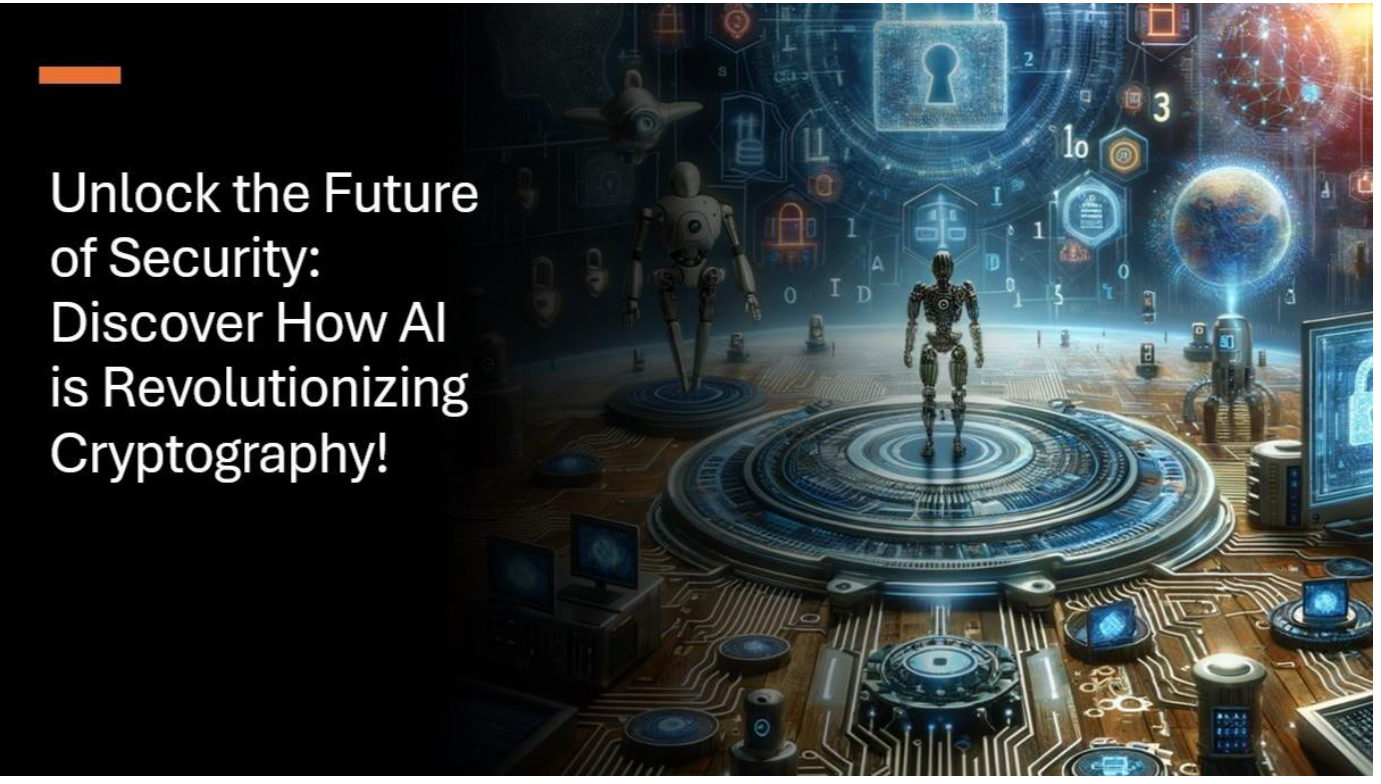
\includegraphics[width=150.99mm,height=215.62mm]{../../images/llm/page_069_img_01.png}%
\end{textblock*}

\end{document}
